% Foliensatz: "AFu-Kurs nach DJ4UF" von DK0TU, Amateurfunkgruppe der TU Berlin
% Lizenz: CC BY-NC-SA 3.0 de (http://creativecommons.org/licenses/by-nc-sa/3.0/de/)
% Autoren: Sebastian Lange <dl7bst@dk0tu.de>
% Korrekturen: Lars Weiler <dc4lw@darc.de>

\documentclass[aspectratio=169]{beamer}

\usepackage[ngerman]{babel} % deutsche Worttrennung etc.
\usepackage[utf8]{inputenc} % UTF8 Text

\usepackage[super, comma, numbers, square, sort]{natbib}

\usepackage{hyperref}       % Hyperref Package für bessere Referenzen (todo)
\hypersetup{
	colorlinks=false,       %   false: boxed links; true: colored links
    %linkcolor=white,       %   color of internal links (change box color with linkbordercolor)
    citecolor=red,          %   color of links to bibliography
    filecolor=white,        %   color of file links
    urlcolor=blue           %   color of external links
}

\usepackage{multirow}
\usepackage{wasysym}  % Math Symbols like \permil
%\usepackage{colortbl}
%\usepackage{subscript}
%\usepackage{caption}
%\usepackage{setspace}
%\usepackage{xcolor}        % benutze CodeListe

% Footnote
%\usepackage{hanging}
%
%\setbeamertemplate{footnote}{%
%  \hangpara{2em}{1}%
%  \makebox[2em][l]{\insertfootnotemark}\footnotesize\insertfootnotetext\par%
%}


%\usepackage{pgf}
%\usepackage{tikz}
%\usetikzlibrary{arrows,automata}
%\usetikzlibrary{positioning}
%
%\tikzset{
%    state/.style={
%           rectangle,
%           rounded corners,
%           draw=black, very thick,
%           minimum height=2em,
%           minimum width=2pt,
%           inner sep=2pt,
%           text centered,
%           },
%}

%\usepackage{listings}
%\lstset{basicstyle=\small, numberstyle=\tiny, extendedchars=true, numbers=left, numbersep=5pt}
%\lstset{showtabs=false, showspaces=false, showstringspaces=false}
%%\lstset{backgroundcolor=\color{white!75!lightgray}, , frame=single}
%%\lstset{backgroundcolor=\color{white}}
%%\lstset{backgroundcolor=none}
%\lstset{keywordstyle=\color{blue!50!gray},  identifierstyle=\color{black}}
%\lstset{commentstyle=\color{green!50!gray}, stringstyle=\color{red!50!gray}}
%\lstset{language=C, fontadjust=true, tabsize=2, breaklines=true}
%\lstset{backgroundcolor=\color{white!75!lightgray}, caption=\lstname, frame=single}
%\lstset{emphstyle=\color{black}\fbox}
%
%% Keine "Listing:"-Caption
%\captionsetup{labelformat=empty,labelsep=none}
%
%% für mathematische Umgebungen
%\usepackage{amsmath,amsfonts,amssymb}
%
%\lstdefinestyle{Bash}{
%language=Bash,
%frame=single,
%rulecolor=\color{black},
%backgroundcolor=\color{gray!50},
%keywordstyle=\color{black},
%identifierstyle=,
%commentstyle=\color{black},
%stringstyle=\color{magenta!65!white},
%showstringspaces=false,
%basicstyle=\footnotesize\ttfamily\color{black},
%numbers=none,
%breaklines=true,
%captionpos=b
%}

%\usepackage{listings}
%
%\lstdefinestyle{basic}{
%    captionpos=t,%
%    basicstyle=\footnotesize\ttfamily,%
%    numberstyle=\tiny,%
%    numbers=left,%
%    stepnumber=1,%
%    frame=single,%
%    showspaces=false,%
%    showstringspaces=false,%
%    showtabs=false,%
%    %
%    keywordstyle=\color{blue},%
%    identifierstyle=,%
%    commentstyle=\color{gray},%
%    stringstyle=\color{magenta}%
%}



% fließende Boxen haben keinen Abstand
%\fboxsep0mm

% inkludiere Creative Commons Helper
%%%%%%%%%%%%%%%%%%%%%%%%%%%%%%%%%%%%%%%%%%%%%%%%%%%%%%%%%%%%%%%%
%% ccBeamer 0.1, 2007-07-02                                   %%
%% Written by Sebastian Pipping <webmaster@hartwork.org>      %%
%% ---------------------------------------------------------- %%
%% Licensed under Creative Commons Attribution-ShareAlike 3.0 %%
%% http://creativecommons.org/licenses/by-sa/3.0/             %%
%%%%%%%%%%%%%%%%%%%%%%%%%%%%%%%%%%%%%%%%%%%%%%%%%%%%%%%%%%%%%%%%


%% Images
\newcommand{\CcImageBy}[1]{%
	
\includegraphics[scale=#1]{texdata/creative_commons/cc_by_30.pdf}%
}
\newcommand{\CcImageCc}[1]{%
	
\includegraphics[scale=#1]{texdata/creative_commons/cc_cc_30.pdf}%
}
\newcommand{\CcImageDevNations}[1]{%
	
\includegraphics[scale=#1]{texdata/creative_commons/cc_dev_nations_30.pdf}%
}
\newcommand{\CcImageNc}[1]{%
	
\includegraphics[scale=#1]{texdata/creative_commons/cc_nc_30.pdf}%
}
\newcommand{\CcImageNd}[1]{%
	
\includegraphics[scale=#1]{texdata/creative_commons/cc_nd_30.pdf}%
}
\newcommand{\CcImagePd}[1]{%
	
\includegraphics[scale=#1]{texdata/creative_commons/cc_pd_30.pdf}%
}
\newcommand{\CcImageSa}[1]{%
	
\includegraphics[scale=#1]{texdata/creative_commons/cc_sa_30.pdf}%
}
\newcommand{\CcImageSampling}[1]{%
	
\includegraphics[scale=#1]{texdata/creative_commons/cc_sampling_30.pdf}%
}
\newcommand{\CcImageSamplingPlus}[1]{%
	
\includegraphics[scale=#1]{texdata/creative_commons/cc_sampling_plus_30.pdf}%
}


%% Groups
\newcommand{\CcGroupBy}[2]{% zoom, gap
	\CcImageCc{#1}\hspace*{#2}\CcImageBy{#1}%
}
\newcommand{\CcGroupByNc}[2]{% zoom, gap
	\CcImageCc{#1}\hspace*{#2}\CcImageBy{#1}\hspace*{#2}\CcImageNc{#1}%
}
\newcommand{\CcGroupByNcNd}[2]{% zoom, gap
	\CcImageCc{#1}\hspace*{#2}\CcImageBy{#1}\hspace*{#2}\CcImageNc{#1}\hspace*{#2}\CcImageNd{#1}%
}
\newcommand{\CcGroupByNcSa}[2]{% zoom, gap
	\CcImageCc{#1}\hspace*{#2}\CcImageBy{#1}\hspace*{#2}\CcImageNc{#1}\hspace*{#2}\CcImageSa{#1}%
}
\newcommand{\CcGroupByNd}[2]{% zoom, gap
	\CcImageCc{#1}\hspace*{#2}\CcImageBy{#1}\hspace*{#2}\CcImageNd{#1}%
}
\newcommand{\CcGroupBySa}[2]{% zoom, gap
	\CcImageCc{#1}\hspace*{#2}\CcImageBy{#1}\hspace*{#2}\CcImageSa{#1}%
}
\newcommand{\CcGroupDevNations}[2]{% zoom, gap
	\CcImageCc{#1}\hspace*{#2}\CcImageDevNations{#1}%
}
\newcommand{\CcGroupNcSampling}[2]{% zoom, gap
	\CcImageCc{#1}\hspace*{#2}\CcImageNc{#1}\hspace*{#2}\CcImageSampling{#1}%
}
\newcommand{\CcGroupPd}[1]{% zoom
	\CcImagePd{#1}%
}
\newcommand{\CcGroupSampling}[1]{% zoom
	\CcImageSampling{#1}%
}
\newcommand{\CcGroupSamplingPlus}[1]{% zoom
	\CcImageSamplingPlus{#1}%
}


%% Text
\newcommand{\CcLongnameBy}{Attribution}
\newcommand{\CcLongnameByNc}{Attribution-NonCommercial}
\newcommand{\CcLongnameByNcNd}{Attribution-NoDerivs}
\newcommand{\CcLongnameByNcSa}{Attribution-NonCommercial-ShareAlike}
\newcommand{\CcLongnameByNd}{Attribution-NoDerivs}
\newcommand{\CcLongnameBySa}{Attribution-ShareAlike}

\newcommand{\CcNote}[1]{% longname
	This work is licensed under the \textit{Creative Commons #1 3.0 License}.%
}


% generelles Thema auswählen
\usetheme{Goettingen} %Berlin spart ohne Sidebar allerdings angenehm Platz
% AnnArbor | Antibes | Bergen | Berkeley | Berlin | Boadilla | boxes | CambridgeUS | Copenhagen | Darmstadt | default | Dresden | Frankfurt | Goettingen | Hannover | Ilmenau | JuanLesPins | Luebeck | Madrid | Malmoe | Marburg | Montpellier | PaloAlto | Pittsburgh | Rochester | Singapore | Szeged | Warsaw

% Farben wählen
\usecolortheme{beetle}
% beaver | beetle | crane | default | dolphin | dove | fly | lily | orchid | rose | seagull | seahorse | sidebartab | structure | whale | wolverine

% Setze alle Farben auf Grau und Weiß
%\definecolor{craneorange}{RGB}{64,64,64}
%\definecolor{craneblue}{RGB}{255,255,255}

% Schriftart wählen
\usefonttheme{default}
% default | professionalfonts | serif | structurebold | structureitalicserif | structuresmallcapsserif

% Innere Themen(Kopf-, Fuß-, Sidebar usw)
%\useinnertheme{default}
\useinnertheme{circles}
% default | inmargin | rectangles | rounded | circles

% Äußere Themen (Anordnung der inneren, grenzen der Folien etc.)
\useoutertheme{infolines}
% default | infolines | miniframes | shadow | sidebar | smoothbars | smoothtree | split | tree

% Deaktiviere Navigations-Symbole ({} -> leer)
\setbeamertemplate{navigation symbols}{}
%\setbeamertemplate{navigation symbols}{\large \ifnum \insertframenumber <10 0\fi\insertframenumber/\inserttotalframenumber\vspace*{0.2ex}}

% Zeige ein Hintergrundbild
\setbeamertemplate{background canvas}{
        \hspace*{-2.0cm}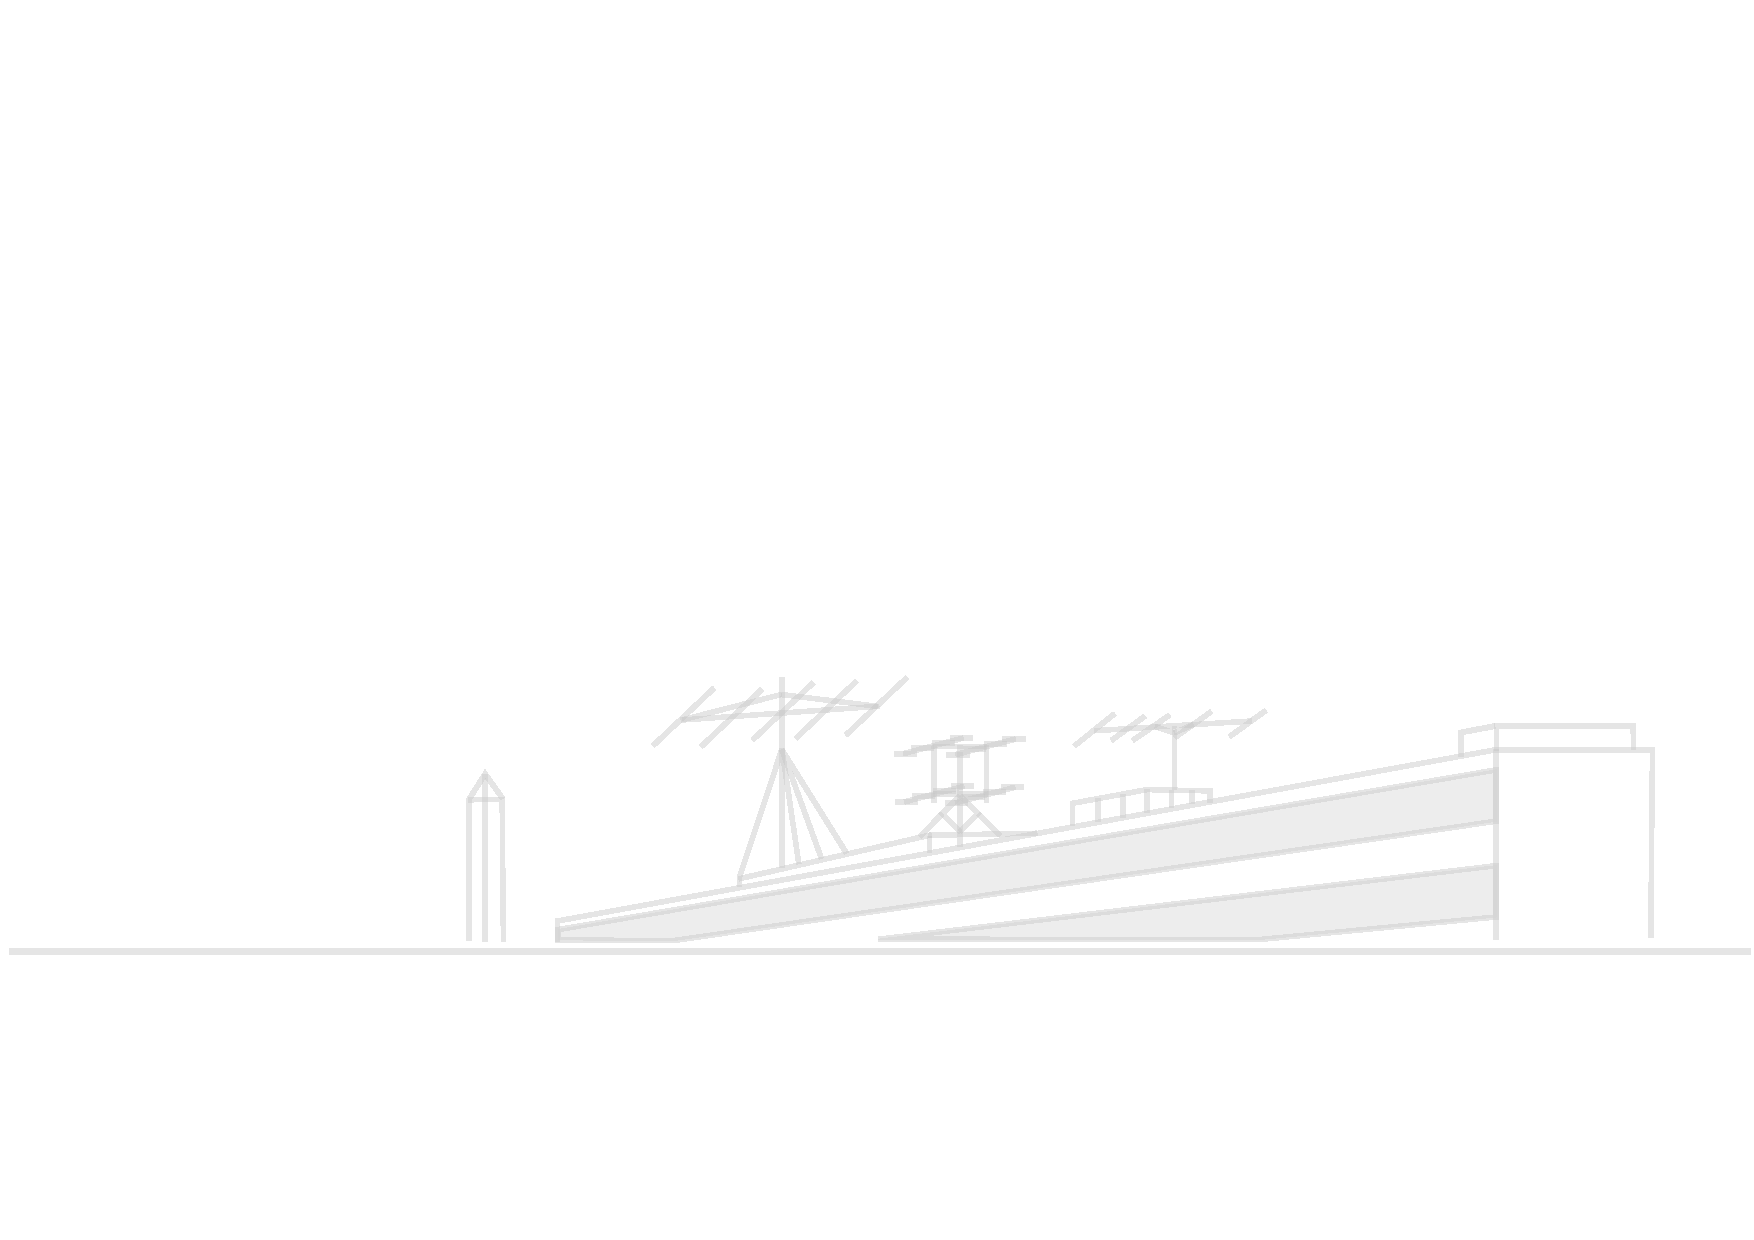
\includegraphics[width=17.8cm]{texdata/dk0tu_rooftop_background.pdf}
}

% Foliennummer einfügen
\setbeamertemplate{footline}[frame number]
%\setbeamertemplate{footline}{}

% Ändere das Zeichen vor jedem item
%\setbeamertemplate{itemize item}{\color{craneorange}$\blacktriangleright$}
%\setbeamertemplate{itemize subitem}{\color{craneorange}$\triangleright$}
%\setbeamertemplate{itemize subsubitem}{\color{craneorange}$\blacktriangleright$}

% Ändert die Blöcke 
\setbeamertemplate{blocks}[rounded][shadow=true]
% default | rounded [shadow=true|false]

%
% Eigene Kommandos
%

% Hack to get natbib and beamer working together. "The beamer user guide suggests
% that only the manual bibliography entry approach is supported"
% on some system it works out of the box, sometimes you need the hack :-(
% so check it --dl7bst
\ifdefined\newblock
    \relax
\else
    \newcommand{\newblock}{}
\fi

% \includedia command to generate png out of a dia file
% NEEDS installed dia and pdflatex option --shell-escape
\newcommand{\includedia}[1]{
    \immediate\write18{/usr/bin/dia #1.dia -e #1_diatmp.png -t png}
}

% RICHIG GROSSER FONT!
\newfont{\bigfont}{cmr10 at 144pt}
\newfont{\smallfont}{cmr10 at 8pt}

% Römische Ziffern
\makeatletter
\newcommand{\rmnum}[1]{\romannumeral #1}
\newcommand{\Rmnum}[1]{\expandafter\@slowromancap\romannumeral #1@}
\makeatother

% Schwarze Überschrift
%\setbeamercolor{frametitle}{fg=black}
%\setbeamercolor{title}{fg=black}

% Item- und Box-Farben
\definecolor{deepBlue}{HTML}{000066}
\setbeamercolor{itemize item}{fg=deepBlue}
\setbeamercolor{itemize subitem}{fg=deepBlue}
\setbeamercolor{description item}{fg=deepBlue}
\setbeamercolor{block title}{fg=deepBlue!100, bg=blue!15}
\setbeamercolor{block body}{fg=black, bg=blue!5}
\setbeamercolor{block title alerted}{fg=deepBlue, bg=red!75}
\setbeamercolor{block body alerted}{fg=black, bg=red!15}
\setbeamercolor*{block title example}{fg=blue!50, bg=blue!10}
\setbeamercolor*{block body example}{fg= blue, bg=blue!5}

%\setbeamercolor{section in head/foot}{parent=palette primary}
%\setbeamercolor{subsection in head/foot}{parent=palette secondary}
%\setbeamercolor{sidebar}{fg=darkblue,bg=yellow!90!orange}
%\setbeamercolor{title in sidebar}{fg=darkblue}
%\setbeamercolor{author in sidebar}{fg=darkblue}
%\setbeamercolor{section in sidebar}{fg=darkblue!10!black}
%\setbeamercolor{subsection in sidebar}{fg=darkblue!50!black}

% Titlepage Infos
\title{AFu-Kurs nach DJ4UF}
\author[DKØTU]{DKØTU\\ \footnotesize{Amateurfunkgruppe der TU Berlin}}
\institute[DKØTU]{\url{http://www.dk0tu.de} }

% PDF-Eigenschaften
\subject{DK0TU-Amateurfunkkurs nach DJ4UF}
\keywords{Amateurfunk Kurs HAM Radio Course CC-BY-NC-SA OpenSource TU Berlin DK0TU}

\subtitle{Betriebstechnik/Vorschriften 10: \\
          Betriebsabwicklung auf Kurzwelle \\[2em]}
\date{Stand 07.01.2016}
 \begin{document}

\begin{frame}
    \titlepage
    \vfill
    \begin{center}
        \ccbyncsaeu\\
        {\tiny This work is licensed under the \em{Creative Commons Attribution-NonCommercial-ShareAlike 3.0 License}.}\\[0.5ex]
         \tiny Amateurfunkgruppe der Technische Universität Berlin (AfuTUB), DKØTU
         %\includegraphics[scale=0.5]{img/DK0TU_Logo.pdf}
    \end{center}
\end{frame}


\section{Einleitung}

\begin{frame}
    \frametitle{Einleitung}

    Was sind die Besonderheiten?

\end{frame}

\section{Allgemeiner Anruf}

\begin{frame}
    \frametitle{Allgemeiner Anruf}

    \begin{itemize}
        \item Vorweg: Auf QRG hören und 2-3x fragen: ``Is this frequency occupied /
              in use?'' wegen toter Zone
        \item QRG nun ``occupied''
        \begin{itemize}
            \item nach Ende des QSOs bleibt die rufende Station
            \item kurze Möglichkeit zur Absprache zum QSY sollte aber gewährt werden
        \end{itemize}
        \item sonst: QSY und wieder hören
    \end{itemize}

\end{frame}

\begin{frame}
    \frametitle{Allgemeiner Anruf: Beispiele}

    SSB: \\
    \emph{CQ this is DKØTU ... DKØTU is calling and standing by} \\
    \emph{CQ this is DKØTU ... and DKØTU is listening}\\[2em]
    
    CW: \\
    \emph{CQ CQ CQ DE DKØTU DKØTU DKØTU} \\[2em]

    \begin{itemize}
        \item QRZ ist kein CQ-Ruf
        \item beim gezielten Anruf einfach die gewünschte Gegenstation ansprechen
        \item alle Rufzeichen im internationalen Buchstabieralphabet verwenden
    \end{itemize}

\end{frame}

\section{Anrufantwort}

\begin{frame}
    \frametitle{Anrufantwort}

    [Call der Gegenstation], this is DKØTU (auch: from)

    \begin{itemize}
        \item in CW immer mit der zuerst gegebenen Geschwindigkeit
        \item bei CW im SSB-Bereich darf auch mit SSB geantwortet werden, ist aber
              unüblich
    \end{itemize}

\end{frame}

\section{Besondere Anrufe}

\begin{frame}
    \frametitle{Besondere Anrufe}

    \begin{itemize}
        \item Weitverkehr: CQ DX (HF: interkontinental, VHF/UHF: ab ca.~300km)
        \item Regionen: z.B. CQ Australia, CQ South America, CQ New Zealand or
              Australia (CW: CQ VK/ZL)
        \item Betriebsarten, Ausbreitungsarten oder Contestabkürzungen:
        \begin{itemize}
            \item CQ Aurora
            \item CQ Sporadic
            \item CQ EME
            \item CQ Contest
            %\item CQ FD
        \end{itemize}
    \end{itemize}
\end{frame}

\begin{frame}
    \frametitle{Besondere Anrufe: Beispiele}

    CQ DL CQ DL de KA2WEU pse k \\[2em]

    CQ FD CQ FD de DH8DAP/p \\[2em]

    A propos \emph{CQ DX}: DX-Pedition ist eine Amateurfunkexpedition zu Ländern
    oder Inseln, die selten im Amateurfunk zu hören sind.

\end{frame}

\section{Spezielle Betriebstechniken}

\subsection{Pile Up}

%TODO Schlechte Slides - mehr Grafik - weniger Text

\begin{frame}
    \frametitle{Pile Up}

    Seltene Stationen wie DX-Peditionen führen fast
    immer zu ``Pile up'':

    \begin{itemize}
        \item gleichzeitiges Anrufen einer selten zu hörenden Station durch
              viele Amateurfunkstellen
    \end{itemize}
\end{frame}

\begin{frame}
    \frametitle{Pile Up: Strategien}

    Split-Betrieb:

    \begin{itemize}
        \item ``5 up'' - 5 kHz höher rufen
              %todo Grafik
        \item im 20m-Band ``tuning 290-300 up'': zwischen 14290 und 14300 kHz rufen
              auch ``split up 290 to 300''
    \end{itemize}

\end{frame}

\begin{frame}
    \frametitle{Pile Up: Strategien}

    Arbeitsreihenfolge:

    \begin{itemize}
        \item ``only number 3, only suffix'', auch Aufsplittung nach Regionen möglich
        \item Listenbetrieb: Gut hörbare andere Station nimmt anrufenden
        Stationen in eine Liste und ruft später diese Stationen zur Aufnahme
        einer Funkverbindung mit der seltenen Station auf
    \end{itemize}

\end{frame}

\subsection{Contest}

\begin{frame}
    \frametitle{Contest}

    % todo aufteilen nach Typ - mehr Bilder

    \begin{itemize}
        \item Betrieb nur in Frequenzbereichen, die nach dem internationalen
          Kurzwellenbandplan und der jeweiligen Contestauschreibung für diesen
          Wettbewerb vorgesehen sind
        \item kurze Durchgänge: Rapport, Exchange, ggf. Locator
        \item viele verschiedene Auswertungssysteme je nach Organisation
        \item z.B. Mobilwettbewerb, COTA (Castle on the Air), \dots
        \item vorher Regelwerk durchlesen
    \end{itemize}

\end{frame}

\begin{frame}
    \frametitle{Contest / Fieldday}

    \begin{itemize}
        \item Fieldday: CQ FD CQ FD de DKØTU/p
    \end{itemize}

    \begin{center}
        % FIXME Kontrast fuer den Beamer suboptimal
        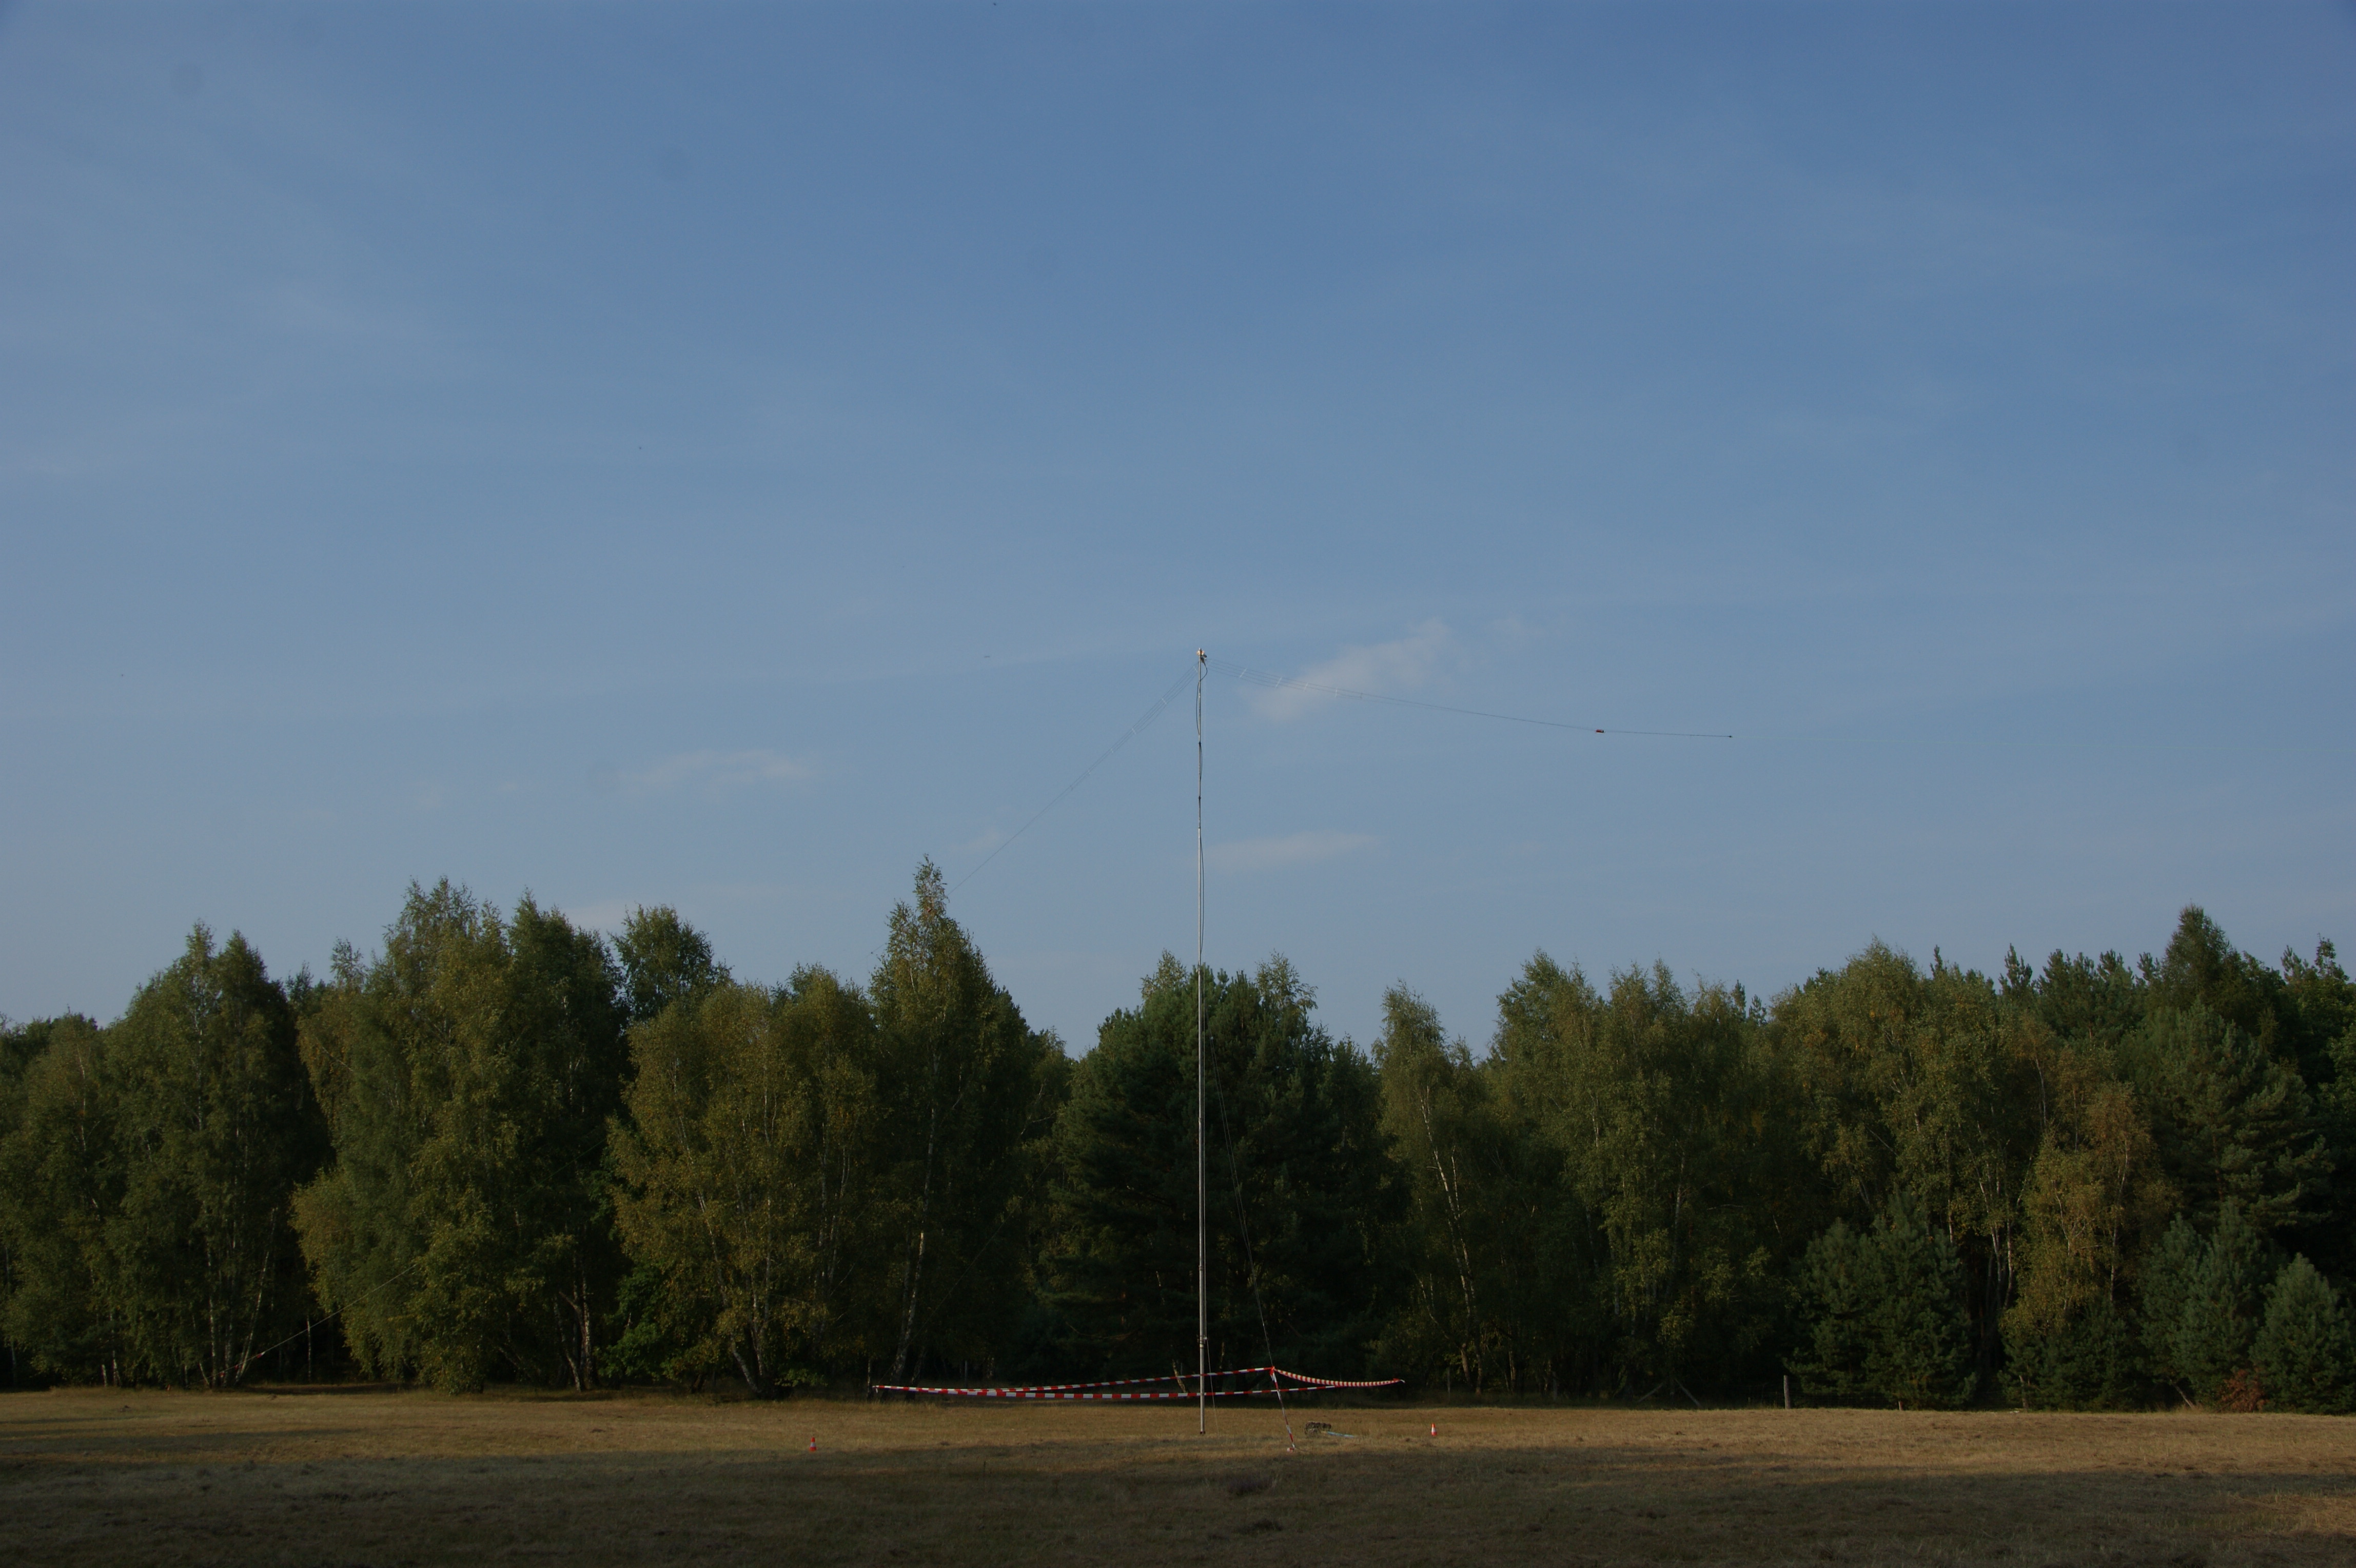
\includegraphics[width=0.8\textwidth,height=.7\textheight,keepaspectratio]{bv10/2014-09-06_160906.jpg}
        \tiny \hyperlink{refs}{\cite{blog}}
    \end{center}

\end{frame}

\begin{frame}
    \frametitle{Contest / ARDF}

    Überbegriff ``ARDF'' (amateur radio direction finding) - Amateurfunkpeilen

    \begin{center}
        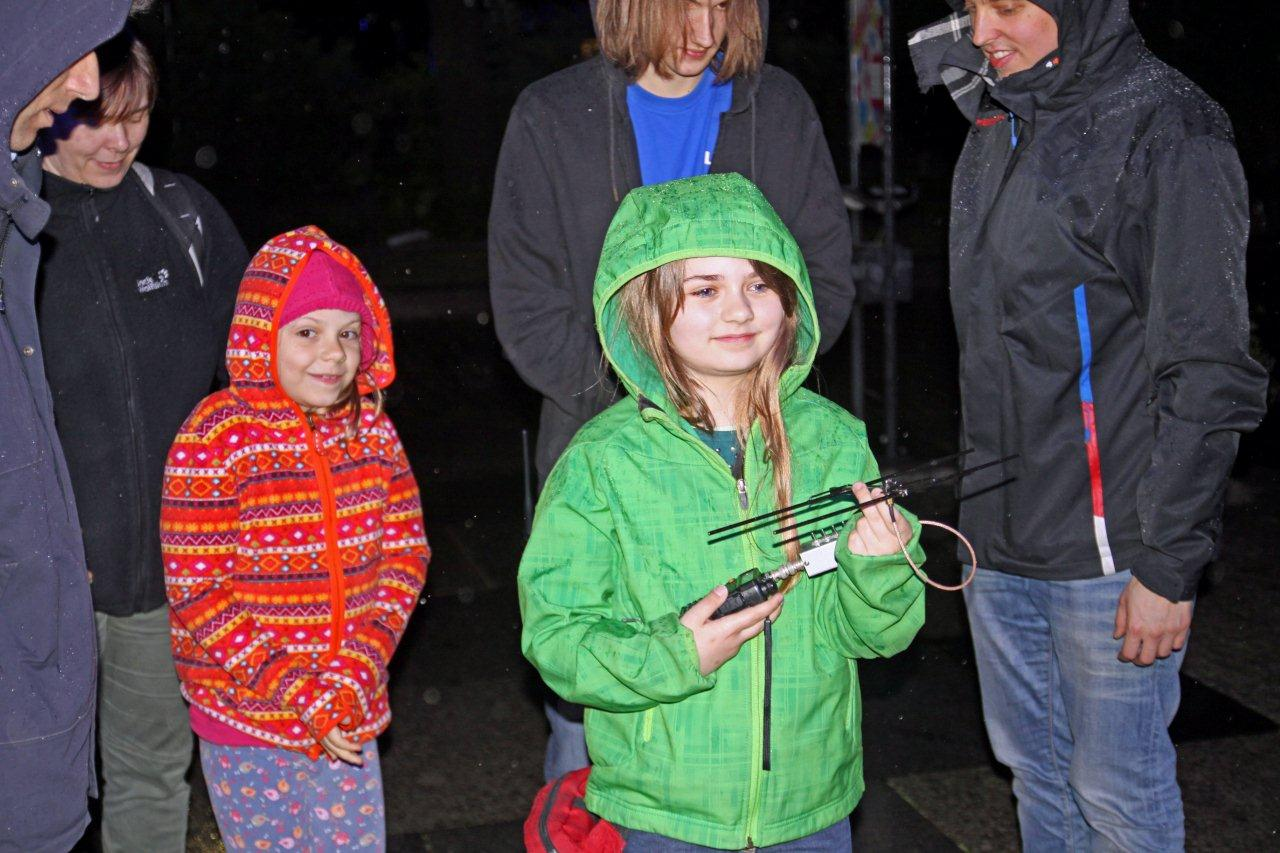
\includegraphics[width=.6\textwidth,height=.5\textheight,keepaspectratio]{bv10/IMG_1910.jpg}
        \tiny \hyperlink{refs}{\cite{blog}}
    \end{center}

    \begin{itemize}
        \item bis zu fünf Sender (Rufzeichen?) bei einer Fuchsjagd - Round Robin
        \item bis zu 16 leistungsschwache beim \emph{Foxoring (``foxhunt and
              orienteering'')} mit Karte
        \item viele weitere Spielarten
    \end{itemize}

\end{frame}

\subsection{Baken}

\begin{frame}
    \frametitle{Baken}

    IARU Bakensystem siehe Kapitel \texttt{BV08}

\end{frame}

\subsection{Notfunk}

% todo Hier sollte noch mehr über den Notfunk innerhalb des Amateurfunks stehen

\begin{frame}
    \frametitle{Notfunk}

    Internationalen Not-, Dringlichkeits- und Sicherheitszeichen:

    \begin{center}
    %\footnotesize
    \begin{tabular}{|l|l|l|}\hline
        \textbf{Signal}       & \textbf{Telegrafie} & \textbf{Phonie} \\ \hline \hline
        Notzeichen            & SOS                 & Mayday          \\ \hline
        Notzeichen (relay\footnote{ausgesendet durch Funkstelle, die selbst nicht in Not ist})
                              & DDD SOS & Mayday Relay \\ \hline
        Dringlichkeitszeichen & XXX                 & Pan              \\ \hline
        Sicherheitszeichen    & TTT                 & Securité         \\ \hline
    \end{tabular}
    \end{center}

    Nur FYI - keine Angst, kein Prüfungsstoff!

\end{frame}

\begin{frame}
    \frametitle{Notfunk: Notsignale}

    \begin{exampleblock}{Dürfen Sie im Notfall eines der Notzeichen SOS oder Mayday gebrauchen?}
      \only<1>{\vspace{1em}}
      \only<2>{Nein, niemals}
    \end{exampleblock}

    \only<2>{
    \begin{quote}
      Die internationalen Not-, Dringlichkeits- und Sicherheitszeichen sollte
      der Funkamateur kennen, da nach §2 Punkt~2 des Amateurfunkgesetztes der
      Amateurfunkdienst von Funkamateuren auch zur Unterstützung von
      Hilfsaktionen in Not- und Katastrophenfällen wahrgenommen
      wird.\footnote{Fragenkatalog BV, Anhang S.~70}
    \end{quote}
    }

\end{frame}

\begin{frame}
    \frametitle{Notfunk: Beispiele aus den Prüfungsfragen}

    \textbf{[BF106] Schiff in Seenot}: ``Ich beobachte die Frequenz und achte
    darauf, ob die Notmeldung von einer Rettungsorganisation bestätigt wird.
    Wenn dies innerhalb einer kurzen Zeit nicht geschieht, rufe ich die Station
    an und biete meine Hilfe an.'' \\[2em]

\end{frame}

\begin{frame}
    \frametitle{Notfunk: Beispiele aus den Prüfungsfragen}

    \textbf{[BF107] Notruf Seefunkstelle/Segelyacht}: ``Ich versuche Kontakt mit
    der Funkstelle aufzunehmen, um den Standort zu erfahren. Danach informiere
    ich die Polizei und bitte um Weitergabe der Information an die zuständigen
    Rettungsorganisationen.'' \\[2em]

    Seefunkstellen sind auf jeden Fall immer Primär. QRG außer im Notfall unter
    keinen Umständen weiterbenutzen!\footnote{Früher wurden Küstenfunkstellen
    eine feste Frequenz zugeteilt, die sie nicht verändern können}

\end{frame}

\begin{frame}
    \frametitle{Notfunk: Frequenzen}

    Aktivitätszentren für Notfunkverkehr nach Empfehlungen der \emph{IARU}:

    \begin{itemize}
        \item 3760 kHz
        \item 7060 kHz
        \item 14300 kHz
        \item 18160 kHz
        \item 21360 kHz
    \end{itemize}

    Welche Bänder sind das? \\[1em]

    Aktivitätszentren innerhalb der IARU-Region 1:\\
    3760 und 7060~kHz! (Prüfungsfrage)

\end{frame}

\begin{frame}
    \frametitle{Nicht nur Notfunk: Zeitangaben}

    \begin{exampleblock}{
        Sie haben am 16. August (Ortsdatum) um 20:00 Uhr mitteleuropäischer
        Sommerzeit (MESZ) von 9J2NG eine Notfunkmeldung aufgenommen und an eine
        Hilfeleistungsorganisation per Telefon weitergemeldet. Die Amateurfunkstelle
        9J2NG hat Sie gebeten, um 23:00 Uhr UTC erneut mit ihr in Verbindung zu
        treten. Welcher Zeitpunkt ist dies in Deutschland?}
        \only<1>{\vspace{1em}}
        \only<2>{01:00 MESZ am 17. August (Ortsdatum)}
    \end{exampleblock}

\end{frame}

\renewcommand{\refname}{Referenzen}

\begin{frame}
    \frametitle{Referenzen/Links}
    \hypertarget{refs}{}
    \footnotesize

    \begin{thebibliography}{}
        \bibitem{dj4uf} Moltrecht B/V 10: \\
                        \url{http://www.amateurfunkpruefung.de/lehrg/bv10/bv10.html}

        \bibitem{blog}  DK0TU Blog: \\
                        \url{http://www.dk0tu.de/blog/2014/09/07_SSB-Fieldday_Dueppeler_Forst/}
                        \url{http://www.dk0tu.de/blog/2014/05/10_LNDW/}
%        \bibitem{wp}    Wikipedia DE: \\
%                        \url{http://de.wikipedia.org/wiki/Frequenzzuteilung} \\
%                        \url{http://de.wikipedia.org/wiki/Amateurfunkband} \\
%                        \url{http://de.wikipedia.org/wiki/Betriebsart_\%28Amateurfunk\%29} \\
%                        \url{http://de.wikipedia.org/wiki/Modulationsart}
%        \bibitem{frqs}  Frequenzplan der BRD von der BNetzA: \\
%                        \url{http://www.bundesnetzagentur.de/DE/Sachgebiete/Telekommunikation/Unternehmen_Institutionen/Frequenzen/Grundlagen/Frequenzplan/frequenzplan-node.html}
%        \bibitem{darc}  Kurzwellenbandpläne der IARU Region 1: \\
%                        \url{http://www.darc.de/referate/hf/bandplaene/}
%        \bibitem{afuv}  Verordnung zum Gesetz über den Amateurfunk: \\
%                        \url{http://www.gesetze-im-internet.de/afuv_2005/}
    \end{thebibliography} 
   
\end{frame}

% Hier könnte noch eine Kontaktfolie stehen

\end{document}

